\label{Elecciones}
\chapter{Análisis Elecciones}
%\agregar{Introducción al Capítulo y Descripción de las secciones - HECHO}

Un sistema de votación exitoso debe cumplir el principal objetivo que es construir la confianza de toda persona involucrada en el proceso: ciudadanos, partidos políticos, gobierno, entre otros. Como posibles alternativas en este proceso, planteadas a nivel mundial, ha sido aplicar distintas técnicas para computarizar parte del proceso de votación. 
Experiencias de implementación de voto electrónico en distintos países obtuvieron impactos de aceptación o con unos cuantos intentos volvieron al sistema electoral tradicional.

\section{Elecciones Internacionales}
%\agregar{Descripción de la seccion - HECHO}
A continuación se eligieron algunos países que implementaron tecnología dentro del proceso de votación. Además se describe brevemente las consecuencias obtenidas y la decisión de cada gobierno en continuar o no utilizando esta técnica.

\subsection{EEUU}
En los años 50 y 60 se utilizaron boletas de tarjetas perforadas, pero este sistema generó mayores problemas al momento del escrutinio como por ejemplo, abolladuras en el papel, se consideraban válidas las marcas sólo si todos los presentes estaban de acuerdo. Las papeletas marcadas con pluma, perforadas más de una vez, perforadas de forma ambigua (por ejemplo, en la línea entre dos partidos) o sin perforación se consideraban votos inválidos.
Como solución a los problemas evidentes de los sistemas de tarjetas perforadas, comienza el auge de los dispositivos de registro electrónico directo de votos (DRE). El uso de dispositivos de votación en EEUU cobró especial relevancia a partir del año 2000, luego de las elecciones presidenciales en donde un gran número de votos no fueron registrados apropiadamente.  \newline
Actualmente, en los distintos estados se emplean diferentes sistemas, que a menudo son utilizados de forma combinada.
%\cambiar{Sin embargo, existen debates sobre los dispositivos utilizados, y han habido causas judiciales en muchos estados respecto a su uso - HECHO}
Sin embargo, existen debates sobre los dispositivos utilizados, y hubo causas judiciales en muchos estados respecto a su uso. Como ejemplo en el estado de Pensilvania se produjeron varios problemas en el equipo de votación electrónica utilizados en Noviembre del 2019, generando suficiente desconfianza en el sistema de votación para las elecciones del 2020. Otro caso es el ocurrido en Nueva Jersey en el que los resultados fueron inmediatos pero el total de votos emitidos no coincidía con la suma de los votos emitidos por partido \cite{eleccionesEEUU}.
En 2002 se aprueba la ley federal Help America Vote Act., que establece un organismo de control denominado Eleccion Assistance Commission (EAC). El EAC conforma un comité técnico para delinear recomendaciones guías para los sistemas de votación, en aspectos de seguridad, testing de usabilidad y establecimiento de estándares y método de prueba para sistemas de votación electrónica. En 2007, la EAC comenzó el proceso de certificación de equipamiento de voto electrónico. Además esta comisión lleva registro de distintos problemas reportados sobre los dispositivos que se usan en la actualidad (Voting System Reports Collecction, 2017) \cite{problemasReportados}.

\subsection{Irlanda}
La primera propuesta de voto electrónico en Irlanda se realizó en 1998 y en el 2000 se introdujo la legislación que permitió el voto eletrónico. Para el 2002, se hicieron las primeras pruebas piloto con el objetivo de extenderlo al resto del pais. Pasaron unos meses para que un informe confidencial del Ministerio del Interior irlandés se filtrara a la prensa: allí se aseguraba que la integridad del proceso electoral no estaba garantizada. Entre otras fallas, el memorando interno que tomó estado público destacaba la posibilidad de que un software malicioso sencillo de programar pudiera generar una pantalla falsa en la máquina para hacer votar incorrectamente al elector. A pesar de este manto de sospecha sobre el sistema, el gobierno irlandés avanzó con el plan de implementación para las eleciones locales y europeas de 2004. Entonces creó la Comisión Independiente de Votación y Escrutinio Eletrónico para que examinara el sistema propuesto. La comisión emitió un informe en el que sostuvo que puede recomendar la utilización del sistema de voto eletrónico pero que, no podía garantizar la seguridad del voto y la rigurosidad del escrutinio. El gobierno no dio marcha atrás con el sistema pero lo puso en suspenso. La inversión que hizo Irlanda en el sistema fue uno de los argumentos principales de las autoridades para no descartar el sistema. Como resultado se registró 52 millones de libras iniciales que se le pagaron a Nedap, y se agregaban los costos de mantenimiento y de actualizacion del sistema (calculando en 700.000 euros anuales y 20.000.000 por única vez).\newline
Finalmente, el 23 de abril de 2009 el entonces ministro anunció que quedaba descartado el sistema de voto electrónico, en base al alto costo de mantenimiento y actualización, sumado a la insatisfacción y sospechas que generó entre los electores. En 2019 se realizó una encuesta al público sobre el uso de elecciones electrónicas consiguiendo un 50\% de aceptación. \cite{eleccionesIrlanda}
\subsection{Holanda}
En el 2008 (un año antes que en el caso irlandés) el gobierno de Holanda había tomado la misma decisión: abandonar el sistema de voto electrónico que había comprado a una empresa local, Nedap. La batalla contra el voto eletrónico en Holanda fue un grupo de activistas informáticos denominado "We don't trust voting computers". Este grupo además de presentaciones judiciales, realizaron una demostración pública en un programa de televisión de las múltiples formas en las que se podía acceder y tomar el control de las máquinas Nedap sin demasiado esfuerzo. En menos de cinco minutos, lograron correr su propio software en una máquina de la empresa y repartir votos de acuerdo a sus preferencias, engañando al elector que utilizaba la máquina. Hasta el día de hoy, Holanda mantiene el sistema de voto por medio de boleta de papel.\cite{netherlands}

%\agregar{citar fuente sumado  artículos científicos por scholar por ejemplo https://ieeexplore.ieee.org/abstract/document/7001135 - HECHO}
\subsection{Estonia}
En las elecciones municipales del 2005, Estonia se convirtió en el primer país del mundo en probar el voto por Internet, remoto. El sistema permite optativamente votar por Internet desde un lugar remoto, la identificación se hace a través del documento nacional de identidad que es una tarjeta inteligente; el voto por Internet es previo al día de la votación dejando al elector modificar su voto las veces que desee, tomándose como válido el último voto. En 2005, casi el 2\% utilizó el mecanismo de voto por Internet y fue creciendo hasta llegar al 30\% de la población en 2015. Las pocas garantías que ofrece sobre el carácter secreto del voto es una de las principales críticas que recibe este sistema. Los expertos consideraron que se debía suspender la aplicación de esta forma de votación, pero las quejas fueron rechazadas por el Comité de Voto por Internet del país y, en 2015, Estonia celebró sus elecciones con el sistema de voto por Internet.\cite{vassil2016diffusion}

%\agregar{citar fuente sumado  artículos científicos scholar - HECHO}

\subsection{Alemania}
A partir de 1998 comenzó a utilizar dispositivos electrónicos de voto (DRE Nedap utilizados en Holanda), comenzando con pruebas pilotos en Colonia y sucesivamente adoptados en distintas ciudades, y generalmente bien aceptadas por la ciudadanía, hasta 2005. En ese año, un par de ciudadanos presentaron una causa ante la Corte Constitucional Alemana, alegando que el uso de máquinas de votación electrónica es inconstitucional y que, dado que son vulnerables, los resultados de las presidenciales de 2005 no son confiables. Un fallo de esta corte dictaminó que el uso de las máquinas Nedap es inconstitucional, aunque no prohíbe el uso de cualquier dispositivo electrónico, sino que requiere que los mismos sean transparentes. Hoy Alemania usa la boleta única en papel.\cite{volkamer2010electronic}

%\agregar{citar fuente sumado  artículos científicos scholar - HECHO %? \url{http://www.brunazo.eng.br/voto-e/textos/CIPPEC-Brunazo.htm}
%\url{http://www2.congreso.gob.pe/sicr/cendocbib/con2_uibd.nsf/1B5274E790C782A1052577BB0075538C/\$FILE/El\_Voto\_Electr\%C3\%B3nico_en_Brasil.pdf}}
\subsection{Brasil}
En 2002 implementó una elección a escala nacional utilizando unos 406.000 dispositivos electrónicos (DRE) en la cual más de 100 millones de votantes emitieron su sufragio. Los reportes de testing de seguridad públicos en 2012 muestran que existen problemas técnicos severos en los dispositivos utilizados. Entre los problemas más relevantes se señalan la inadecuada protección del secreto del voto, el uso inapropiado de encriptación y algoritmos de criptografía obsoletos, modelos de ataques inadecuados centrados en atacantes externos cuando los ataques internos presentan un riesgo mucho mayor, adopción de un proceso de desarrollo de software defectuoso y verificación de integridad insuficiente.\cite{brunazo2005voto}

%\agregar{Sección Experiencias en Argentina y como Subsecciones cada una de las experiencias - HECHO}
\section{Experiencias en Argentina}
%\agregar{En el país hay experiencias de sumar tecnología en Elecciones Municipales, Provinciales y Nacionales, con diferentes niveles de aceptación, metodologías y aplicado a distintas fases del proceso.  En algunas implementaciones solo se agrega tecnología a la fase de Comunicación de Resultados y en otros a todo el procesos desde la fase de Emisión del voto.....  En las siguientes sub-secciones se describen algunas experiencias a nivel Municipal, Provincial y Nacional - HECHO}
Además de las experiencias de implementación de voto electrónico en distintos países con variadas técnicas, tenemos ejemplos a nivel nacional en Elecciones Municipales, Provinciales y Nacionales. Estas experiencias tuvieron diferentes niveles de aceptación, metodologías y distintas fases del proceso de votación involucraron tecnología. En las siguientes subsecciones se describen ejemplos de experiencias en Argentina.

%\cambiar{Elecciones Municipalidad de Las Grutas - HECHO}
\subsection{Elección Municipal de Las Grutas}
El 16 de diciembre de 2007 se utilizaron 4 urnas electrónicas de la firma Altec Sociedad del Estado (Rio Negro) en la localidad de Las Grutas (Argentina). Durante la jornada electoral, ocurrieron casos donde la urna no habilitaba al votante siendo que en el padrón en papel figuraba, siendo un claro atentado contra el secreto del voto. Otro de los problemas fueron máquinas que se trababan y al trabarse el papel utilizado dejaba en evidencia la elección del votante. La utilización de estas urnas electrónicas se implementó a pesar que el 10\% de los habitantes del lugar elevaran al superior tribunal de justicia la no obligatoriedad de este sistema. \cite{eleccionesLasGrutas}
%\cambiar{Elecciones Provinciales Neuquén - HECHO}
\subsection{Elecciones Provinciales de Neuquén en 2019}
El 10 de Marzo de 2019, Neuquén realizó la elección para gobernador y vicegobernador por medio del sistema de boleta electrónica, y con el sistema tradicional en papel en mesas con menor concurrencia. Se utilizaron máquinas BUE como se muestra en la figura \ref{fig:maquinasBUE}, las cuales eran manipuladas directamente por el votante, imprimiendo su votación sobre una boleta electrónica utilizando un chip que luego es usado para el escrutinio de cada mesa. El proceso de votación se conformó de las características en el proceso:
%\cambiar{y con el sistema tradicional en papel solo ....\% \url{http://200.70.33.130/images2/Electoral/CP_10-03-2019/Info_general/datos_generales_de_la_eleccion.pdf} - HECHO}
\begin{figure}
\begin{center}
  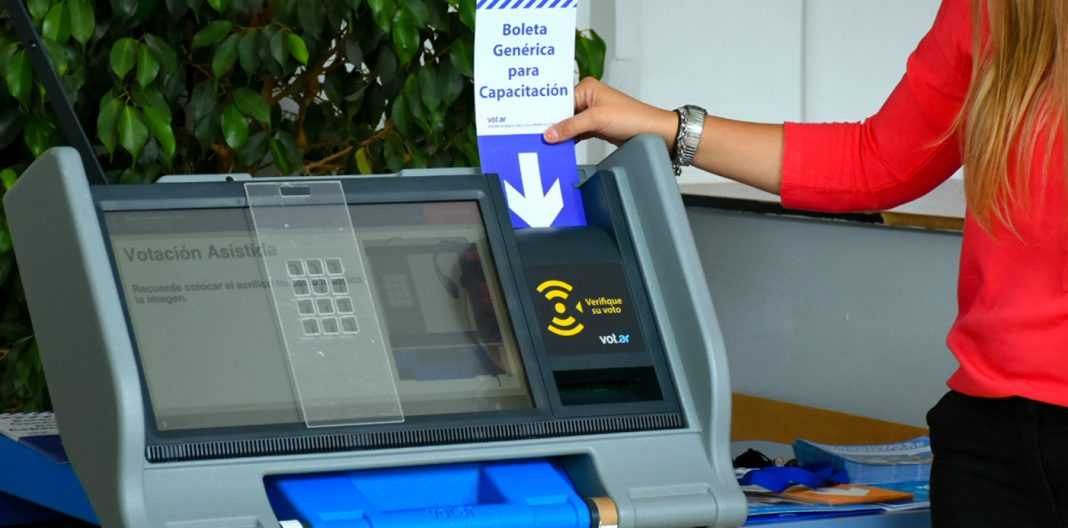
\includegraphics[scale=0.4]{img/Maquina_BUE.jpg}
  \caption{Máquina utilizada en las elecciones de Neuquén}
  \label{fig:maquinasBUE}
\end{center}
\end{figure}
\begin{itemize}
    \item Votación utilizando la máquina electrónica.
    \item Conteo utilizando la maquina electrónica y las boletas electrónicas.
    \item Envío de datos de las escuelas con la máquina electrónica utilizando el certificado generado de cada escrutinio de la mesa.
    \item Resultados provisorios
\end{itemize}

\newline Sobre estas elecciones se obtuvieron los siguientes datos \footnote{http://200.70.33.130/images2/Electoral/CP_10-03-2019/Info\_general/datos\_generales\_de\_la\_eleccion.pdf}:
\begin{itemize}
    \item 493.760 neuquinos estuvieron habilitados para votar, de los cuales se contabilizó una participación del 78.44%
    \item 1.504 mesas distribuidas en 283 escuelas, de las cuales 191 trabajaron con el sistema BUE (Boleta Única Electrónica), 86 con el sistema tradicional de papel y 6 escuelas tuvieron ambos sistemas
\end{itemize}

Se obtuvieron los datos de estas elecciones utilizando la técnica de Web Data Scraping, esta técnica se basa en un proceso de extracción y combinación de contenido alojado en la Web de manera sistemática. Se extraen los datos de interés y se lo estructura como se lo desee \cite{glez2014web}.

Para aplicar esta técnica se utilizó un pequeño script para extraer y estructurar la información obtenida a través de una API, provista por la provincia de Neuquén, hacia una estructura útil para nuestro propósito. Se analizaron los datos y se puede ver la evolución de la carga de mesas en el gráfico \ref{graf:porcentajeNeuquen} y su velocidad de carga en el gráfico \ref{graf:velocidadNeuquen}. Como se puede ver, los datos fueron agrupados en fracciones de 10 min durante todo el proceso de escrutinio.

\begin{figure}[h!]
  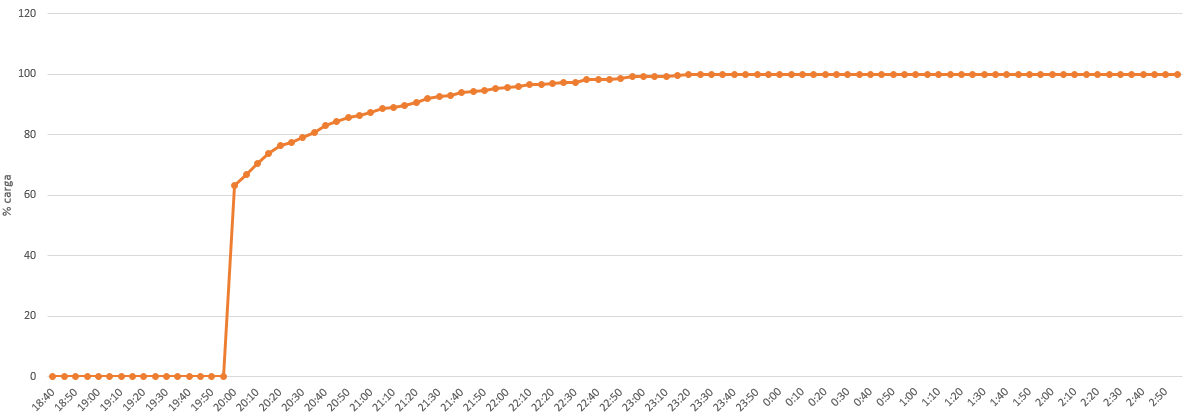
\includegraphics[width=1\textwidth]{img/fOI0sHj9ac.png}
  \caption{Porcentaje de mesas cargadas - Neuquén (2019)}
  \label{graf:porcentajeNeuquen}
\end{figure}

\begin{figure}[h!]
  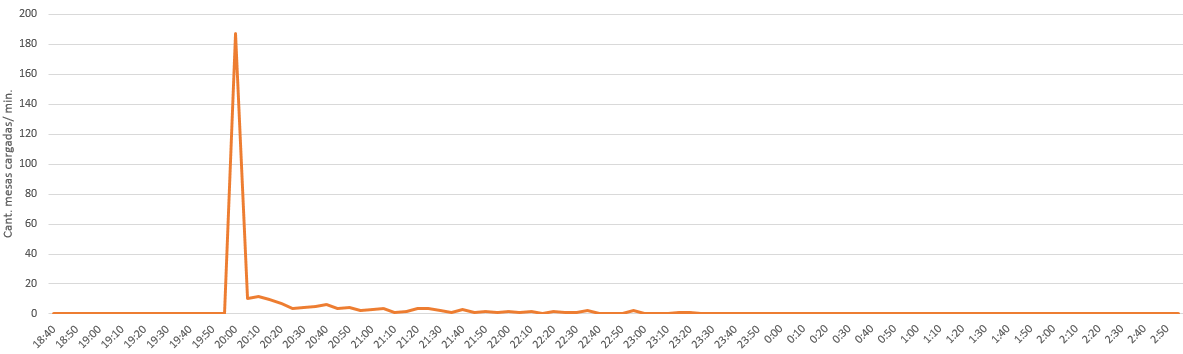
\includegraphics[width=1\textwidth]{img/QOsSnICbyL.png}
  \caption{Velocidad en carga de mesas - Neuquén (2019)}
  \label{graf:velocidadNeuquen}
\end{figure}


\subsection{Elecciones Provinciales de Rio Negro en 2019}
El 7 de Abril de 2019, Río Negro realizó la elección para gobernador y vicegobernador por medio del sistema tradicional de votación en papel. Cada votante contendrá en su sobre su lista y/o listas elegida en papel y, el escrutinio se realiza manualmente enviándose los datos desde cada escuela por medio de telegramas. El proceso de votación para esta elección se conformó de los siguientes elementos:
\begin{itemize}
    \item 7 listas candidatas que el elector puede elegir.
    \item 546.067 electores habilitados, esto quiere decir que se prepararon 546.000 sobres aproximadamante, uno por cada elector.
    \item 1646 mesas, esto implica la misma cantidad de urnas.
\end{itemize}
Teniendo estos datos se puede concluir que sólo para elecciones de gobernador y vice se utilizaron aprox. 3.822.000 papeles, 7 listas preparadas para 546.000 electores. De igual manera que en las elecciones de Neuquén, se obtuvieron los datos de las elecciones utilizando la técnica de web scraping, obteniendo una evolución de carga de mesas representado en el gráfico \ref{graf:porcentajeRioNegro} y su velocidad de carga en el gráfico \ref{graf:velocidadRioNegro}. Como se puede ver, los datos fueron agrupados en fracciones de 10 min durante todo el proceso de escrutinio.

%\agregar{explicación de que se trata y cita a algún artículo científico - HECHO}

%\cambiar{Caption de \ref{graf:porcentajeRioNegro}  \ref{graf:velocidadRioNegro} las de Córdoba también aclarando de que elecciones es y de cuando es.   De neuquen no hay gráfico? - HECHO} 
\begin{figure}[h!]
  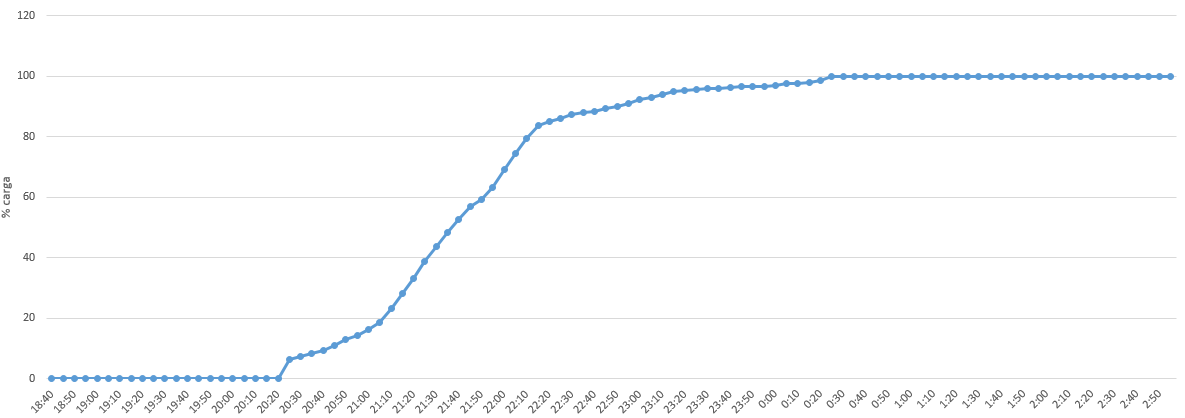
\includegraphics[width=1\textwidth]{img/sAveHlGEkX.png}
  \caption{Porcentaje de mesas cargadas - Rio Negro (2019)}
  \label{graf:porcentajeRioNegro}
\end{figure}

\begin{figure}[h!]
  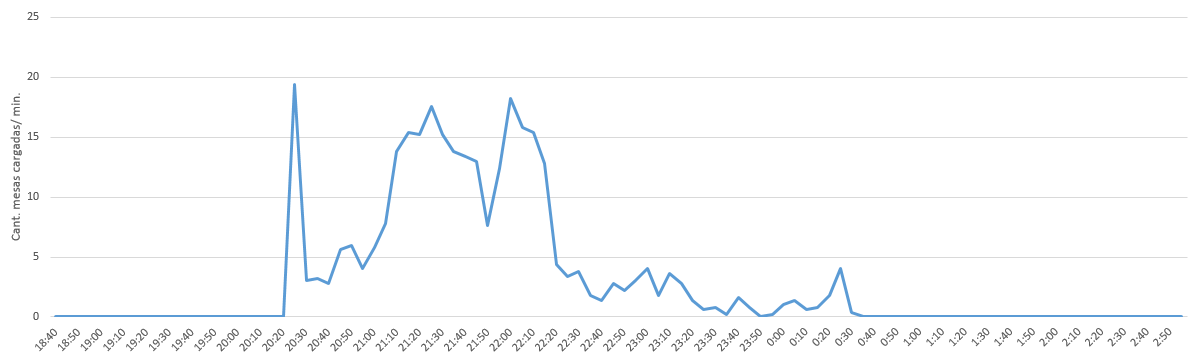
\includegraphics[width=1\textwidth]{img/8w25IVQD5U.png}
  \caption{Velocidad en carga de mesas - Rio Negro (2019)}
  \label{graf:velocidadRioNegro}
\end{figure}

\subsection{Elecciones Provinciales de Córdoba}
%\cambiar{No es boleta única papel? hay una impresora en cada mesa? - HECHO}
El 12 de Mayo de 2019, Córdoba realizó la elección para gobernador, legisladores,  candidatos a ocupar el tribunal de cuentas provincial, y en algunas localidades se renovaron autoridades municipales, por medio del sistema de boleta única de sufragio (BUS) \cite{cortiboleta}. Este método consta de una única boleta impresa con todos los cargos y candidatos sobre el cual el votante indica su elección dentro de esta boleta, el cual se ingresa en la urna. En las columnas se organizan cada uno de los cargos y en las filas se listan los espacios políticos como se puede ver en la imagen \ref{graf:BUSCordoba}.
\begin{figure}[h!]
  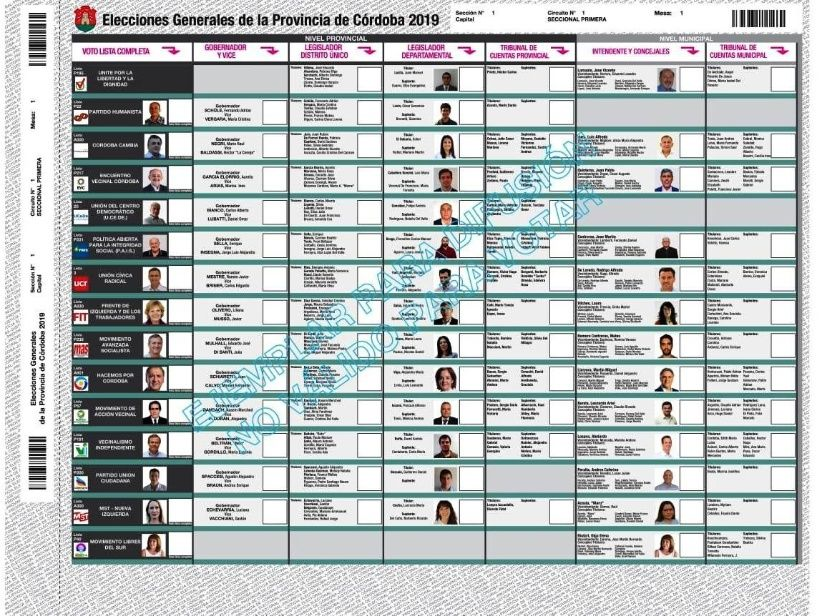
\includegraphics[width=1\textwidth]{img/boletaunica-cordoba.jpg}
  \caption{Ejemplo de la Boleta Única de Sufragio (BUS)}
  \label{graf:BUSCordoba}
\end{figure}
Luego el escrutinio se realizó de manera manual enviándose los datos de cada escuela por medio de telegramas. El proceso de votación para esta elección se conformó de los siguientes elementos: 
\begin{itemize}
    \item 13 listas candidatas para gobernador que el elector puede elegir
    \item 2.889.973 electores habilitados, esto quiere decir que se prepararon 2.889.000 boletas aproximadamente, uno por cada elector
    \item 8654 mesas
    \item 320 millones de pesos costó este sistema. 
\end{itemize}
%\cambiar{3.000.000 de boletas un poco más por las dudas. - HECHO}
Debido a que sólo se utiliza una boleta por elector, se puede concluir que sólo para elecciones de gobernador y vice se utilizaron cerca de 3.000.000 boletas en papel. Como se puede ver su resultado es mucho menor a las elecciones de Río Negro, aún teniendo éste cerca de un 20\% de electores habilitados a comparación de Córdoba. De igual manera que en las elecciones de Neuquén y Río Negro, se obtuvieron los datos de las elecciones utilizando la técnica de Web Data Scraping, obteniendo una evolución de carga de mesas representado en el gráfico \ref{graf:porcentajeCordoba} y su velocidad de carga en el gráfico \ref{graf:velocidadCordoba}. Como se puede ver, los datos agrupados en fracciones de 10 min. durante todo el proceso de escrutinio.

\begin{figure}[h!]
  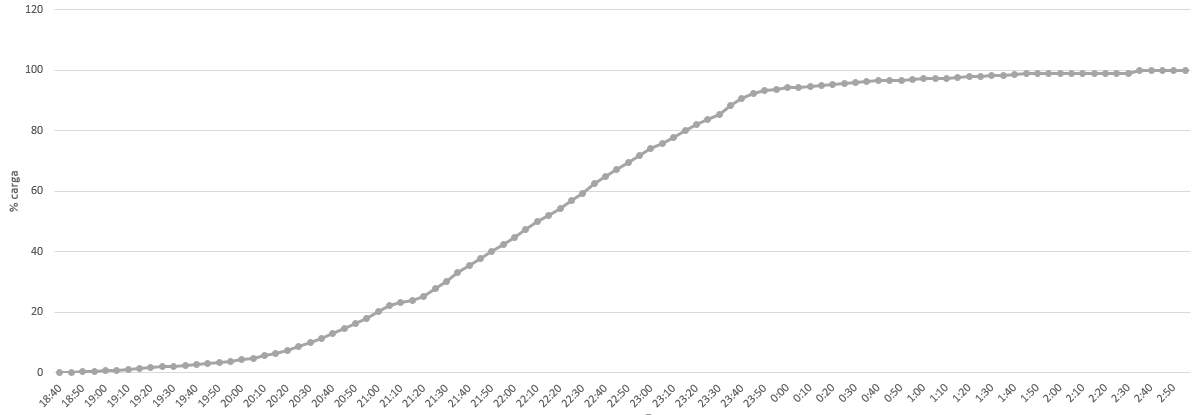
\includegraphics[width=1\textwidth]{img/E4YqKc5Tcu.png}
  \caption{Porcentaje de mesas cargadas - Córdoba (2019)}
  \label{graf:porcentajeCordoba}
\end{figure}

\begin{figure}[h!]
  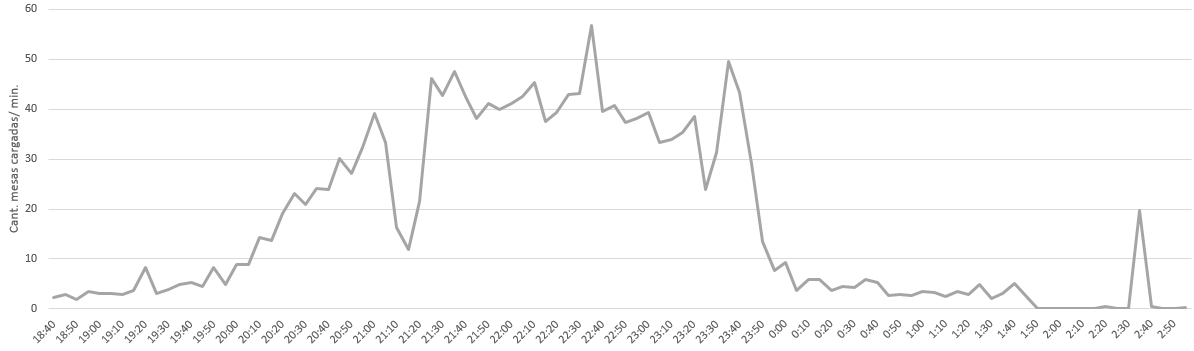
\includegraphics[width=1\textwidth]{img/9rEiyqeSFw.png}
  \caption{Velocidad en carga de mesas - Córdoba (2019)}
  \label{graf:velocidadCordoba}
\end{figure}

%\cambiar{llevaría esta sección como subsección de Experiencias en Argentina - ???}
\subsection{Sistema Escrutinio Nacional 2019}
En 2019 se utiliza el sistema llamado SmartTally \footnote{https://www.smartmatic.com/es/elecciones/elecciones-manuales/smarttally/}, que consta en el envío de telegramas directo desde el establecimiento hacia los centros de cómputos de la Dirección Nacional Electoral (DINE), que depende del Ministerio del Interior de la Nación. Con el objeto de agilizar el trámite que es llevado a cabo por el Correo Argentino. Cada establecimiento consta de una impresora multifunción, conexión a internet y un equipo que permite la conexión y monitoreo del envió exitoso de los telegramas. \newline
Este sistema fue usado en las elecciones las PASO (11 de Agosto de 2019) y Elecciones Naciones (27 de Octubre de 2019).
%\cambiar{Sacar la siguiente línea o bien describir el proceso - HECHO}

Polémicas al usar este tipo de sistema:
\begin{itemize}
    \item Auditabilidad del Software: Se requirió que la empresa ponga a disponibilidad el software usado para su investigación, a modo de reconocer posibles fallas. Frente a este pedido el Gobierno notifica que no es posible ya que el software es alquilado y la empresa dueña se niega a entregar este producto.\cite{auditabilidadSmartmatic}
    \item Seguridad frente a ataques externos: Javier Smaldone presentó vulnerabilidades en el software de conversión de formato de los ``telegramas'' electorales poniendo en riesgo la integridad del proceso. \cite{seguridadSmartmatic}
    \item Transparencia: Debido a que este sistema consta de dos etapas en el proceso de escrutinio, existe cierta desconfianza entre los datos cargados por cada transmisión exponiendo los resultados provisorios y el resultado final luego de ser validado dentro de los 10 días como indica el código electoral. Este primer resultado podría generar datos ganadores que luego no son así en el resultado final. \cite{rnEscrutinioProvisorio}
\end{itemize}



%\agregar{Sección Análisis de la utilización del Tecnología en Elecciones - ??}
\section{Análisis de la utilización de Tecnología en Elecciones}
El año 2019 fue un año ideal para el análisis de sistemas electoral nacionales, se realizaron múltiples elecciones a nivel municipal, provincial y nacional. Además de las magnitudes en cada elección se implementaron distintas técnicas en el proceso de elección. Esto permitió tomar experiencias y realizar una comparación de velocidad de publicación de resultados. A continuación de describen las elecciones provinciales en Neuquén, Rio Negro y Córdoba cuyas elecciones utilizaron diferentes sistemas. Con respecto a la ciudad de Neuquén Capital se realizó una encuesta del nivel de aceptación, confianza y conocimiento del sistema BUE utilizado en tres ocasiones anteriores a este año, por lo tanto, existía un aprendizaje de la población.

%\agregar{Durante el año 2019 en el país se realizaron múltiples elecciones a nivel municipal, provincial y nacional, situación que ha sido favorable para comparar diferentes sistemas.   En las siguiente sub-secciones se realizan una comparación de la velocidad de publicación de resultados de elecciones provinciales utilizando diferentes sistemas y un análisis mediante encuesta del nivel de aceptación, confianza y conocimiento del sistema BUE utilizado en las elecciones Municipales de la Ciudad de Neuquén - HECHO}

%\cambiar{Análisis comparativo de la velocidad de publicación de Resultados de elecciones Provinciales en Neuquén, Córdoba y Río Negro - HECHO}
\subsection{Análisis comparativo en Elecciones Provinciales de Neuquén, Córdoba y Río Negro en 2019}
A través de resultados almacenados en \textit{datosoficiales.com} se consiguieron los datos de cada elección detallada en las secciones anteriores de Neuquén, Río Negro y Córdoba.   \newline
En estas tres experiencias, las provincias contrataron a la empresa MSA \footnote{MSA \url{https://www.msa.com.ar/}} utilizando distintas técnicas, esto es aplicando tecnología en diferentes fases y logrando los resultados como se muestra en la tabla \ref{tab:comparativa}.
%\agregar{En las tres experiencias, las Provincias contrataron a la empresa MSA \footnote{MSA \url{https://www.msa.com.ar/}} utilizando diferentes técnicas, aplicando tecnología en diferentes faces y logrando diferentes resultados como muestra la Tabla \ref{tab:comparativa}.}
\begin{table}[]
    \centering
    \begin{tabular}{c|c|c|c}
         Provincia & Neuquén& Río Negro & Córdoba   \\
         \hline
         Técnica utilizada& BUE & Tradicional & BUS \\
         \hline
         Electores& & & \\
         \hline
         Mesas& & & \\
         \hline
         Tecnología aplicada a& &Comunicación de Resultados & Comunicación de Resultados \\
         \hline
         *Computado el 80\% & & & \\
         \hline
    \end{tabular}
    \caption{Comparativa de diferentes métodos utilizados en elecciones provinciales de 2019}
    \label{tab:comparativa}
\end{table}


A partir de esto, en el gráfico \ref{fig:velocidad} se puede observar la velocidad comparativa de cada carga en las tres provincias, y en el gráfico \ref{fig:acumulado} se representa el porcentaje acumulado durante el periodo de escrutinio. En estos gráficos, la linea naranja representaría las elecciones utilizando BUE, la linea gris las elecciones utilizando Boleta Única y la linea azul es el resultado de las elecciones tradicionales con boletas partidarias de papel. \newline
A primera impresión se puede observar la notable velocidad de carga en la provincia de Neuquén en los primeros minutos de las 20:00 hs., satisfaciendo el objetivo de rapidez de las máquinas BUE. Sin embargo, se reduce su velocidad hasta completar la totalidad de las mesas. Por otro lado, la provincia de Córdoba, por medio de la Boleta Única logra una velocidad constante de carga hasta completar la totalidad de las mesas. Como se puede observar en el gráfico \ref{fig:acumulado} la completitud de las mesas escrutadas se logra con poca diferencia de horas, dando a notar que aplicando tecnología en cualquier etapa del escrutinio no genera un impacto notable en la velocidad de los resultados. 
Al igual que estas elecciones sobre estas provincias, se intentó aplicar la técnica de Web Data Scraping para evaluar la velocidad de carga en las elecciones nacionales PASO y Generales de 2019. Sin embargo, no se logró obtener datos útiles para nuestro propósito ya que estos datos no contenían fechas y horas de publicación de cada mesa. Igualmente, en las Elecciones Generales 2019 a las 21:00 hrs. se logró publicar un 80\% del total de mesas, lo que muestra una técnica con muy buenos tiempos de velocidad de publicación de resultados.
%\agregar{Se realizó el mismo proceso de scraping para evaluar la velocidad de carga de las elecciones nacionales PASO y Generales 2019, pero el sistema de publicación de resultados no ofrecía el la fecha y hora en que se publicó cada mesa.  Igualmente, la segunda vez que se utilizó el sistema en las Elecciones Generales 2019, a las 21:00 ya había un 80\% de las mesas publicadas lo que muestra un método con muy buenos tiempos de velocidad de publicación de resultados...... ???}
\newline


\begin{figure}[h!]
  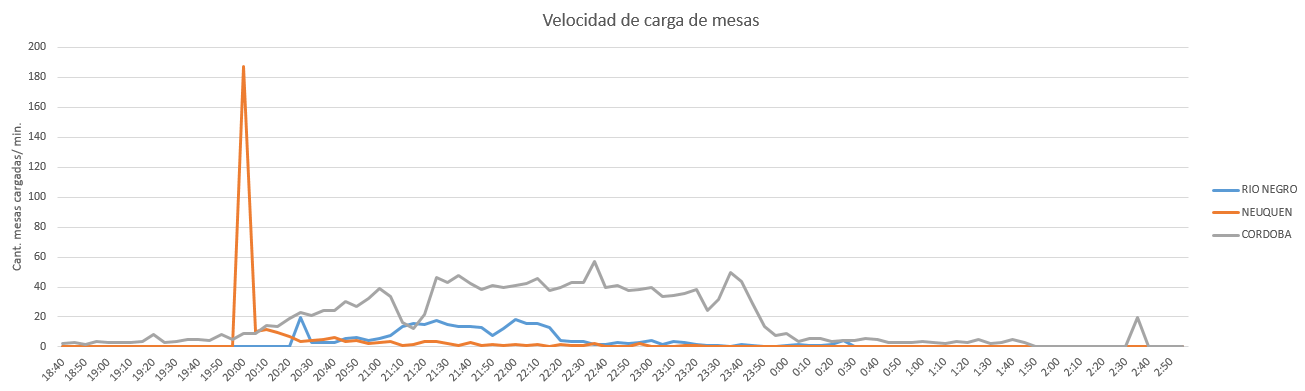
\includegraphics[width=\textwidth]{img/grafico_velocidad_carga.png}
  \caption{Velocidad de Cargas de mesas}
  \label{fig:velocidad}
\end{figure}
\begin{figure}[h!]
  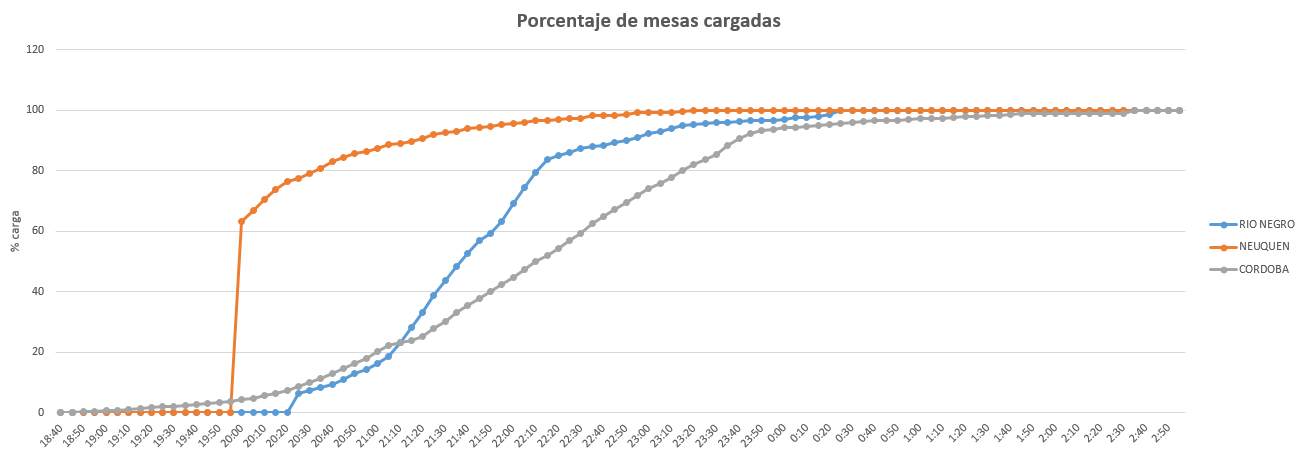
\includegraphics[width=\textwidth]{img/carga_mesas.png}
  \caption{Porcentaje de mesas cargadas}
  \label{fig:acumulado}
\end{figure}

Otra elección que logró implementar un sistema electoral tradicional sin intervención tecnólogica utilizando la boleta única fue en San Carlos de Bariloche el 1 de Septiembre del 2019 \footnote{Noticia: https://www.anbariloche.com.ar/noticias/2019/08/24/70978-elecciones-municipales-como-se-vota-con-la-boleta-unica}. Una característica que puede generar inconvenientes de este tipo de boleta es el tamaño que puede conseguir, ya que tiene que contener todas las listas disponibles. Por ejemplo, en las elecciones de Córdoba se tiene un tamaño de 40cm de alto por 47 cm de ancho como modelo general, este tamaño podría extenderse en municipios o dependiendo de la cantidad de partidos o alianzas que se presenten \cite{boletaUnicaTamanio}. \newline
Por otra parte, el sistema BUE consta de una boleta con un chif RFID sobre la cual se escribe la voluntad del votante. Dentro del modelo de referencia consta de las fases de Emisión del voto y además esta boleta es utilizada para la fase posterior de Escrutinio de la mesa. A pesar del debate impulsado por varias instituciones en contra del uso de este método, varios municipios lo utilizaron. Un inconveniente que puede albergar este sistema es la limitación en pantalla. Una pantalla dispone de 18 lugares para ubicar a los candidatos. Con el uso de listas colectoras se llegaron a multiplicar las listas. La disposición de los candidatos en la pantalla de estas máquinas puede afectar la accesibilidad de los electores al reducirse el tamaño de cada cuadricula. Como ejemplo, en Plottier \cite{lmncolectoras} se dispusieron 29 candidatos a intendencia de la ciudad y 26 en Neuquén. 
%\cambiar{Análisis de opinión pública sobre las elecciones en Neuquén Capital - HECHO}
\subsection{Análisis sobre la opinión pública sobre las elecciones en Neuquén Capital}
En las elecciones a intendente en Neuquén Capital el día 22 de Septiembre de 2019 se realizó una encuesta con la intención de conocer las opiniones de los votantes. Al ser un municipio que luego de 4 elecciones utilizando el sistema BUE, sería una buena muestra de votantes con experiencia sobre este dispositivo, o es lo que se espera. Esta actividad involucró votantes de cuatro escuelas repartidas en puntos importantes de la ciudad. Las escuelas encuestadas fueron Esc. nº201 (Barrio Centro), nº 40 (Barrio San Lorenzo), nº 20 (Barrio Don Bosco) y nº 103 (Barrio Confluencia) logrando encuestar 145 personas en total. \newline
El objetivo de esta encuesta fue conocer el nivel de aprendizaje de los votantes sobre este nuevo sistema y en respuesta a su uso, cuánta confianza y facilidad les resulta este medio de votación. A cada votante se le hacían cinco preguntas con opciones de respuesta para que el cuestionario se logre hacer en no más de 5 minutos. Las preguntas fueron:
\begin{enumerate}
    \item ¿La persona encuestada votó?
    \item ¿La persona encuestada leyó su boleta impresa?
    \item ¿La persona encuestada verificó su boleta utilizando el lector de chip RFID?
    \item ¿A la persona encuestada le resulta simple votar con la boleta BUE?
    \item ¿La persona encuestada confía en el sistema de votación utilizada?
\end{enumerate}

Cabe aclarar que esta encuesta se realizó a 100 metros de distancia de la escuela por Código Electoral y como se puede observar las preguntas estaban enfocadas a cómo realizar la votación, no se hicieron preguntas personales sobre su voto. Se decidió subdividir las muestras por edad generacional, por lo tanto, se encuadra cada votante dentro de las categorías
\begin{itemize}
    \item Z: Personas nacidas a partir del 2000, representado en la tabla como menores a 25 años aprox.
    \item Y: Personas nacidas entre 1980-1999, representado en la tabla con edades entre 25 y 39 años aprox.
    \item X: Personas nacidas entre 1965-1979, representado en la tabla con edades entre 39 y 55 años aprox.
    \item BG: Personas nacidas entre 1946-1964, representado en la tabla con edades mayores a 55 años aprox.
\end{itemize}
Al finalizar las encuestas se obtuvieron los datos de la tabla \ref{tab:encuesta} donde se contabilizan la cantidad de personas que respondieron a cada opción para cada pregunta.
\begin{table}[h!]
\caption{Resultado sobre los encuestados}
\begin{center}
\resizebox{\textwidth}{!}{
\begin{tabular}{ |c|c|||c|c|c||c|c|c||c|c|c||c|c|c|c| } 
 \hline
 \multirow{2}{4em}{Pregunta} & \multirow{2}{3em}{Generación} & \multicolumn{3}{|c||}{Escuela nº201} & \multicolumn{3}{|c||}{Escuela nº40} & \multicolumn{3}{|c||}{Escuela nº20} & \multicolumn{3}{|c|}{Escuela nº103} & \multirow{2}{3em}{Total}\\
  & &SI & MASO & NO & SI & MASO & NO & SI & MASO & NO & SI & MASO & NO & \\ 
 \hline
 \multirow{4}{3em}{¿Votó?} & Z < 25 & 2 & & & 7 & & & 4 & & & 5 & & & 18 \\ 
 & 25 <= Y < 39 & 8 & & & 12 & & & 12 & & & 4 & & & 36\\ 
 & 39 <= X < 55 & 15 & & & 12 & & & 13 & & & 23 & & & 63 \\
 & 55 <= BG & 12 & & & 5 & & & 7 & & & 4 & & & 28\\ 
 \hline \hline
 \multirow{4}{3em}{¿Leyó?} & Z < 25 & 1 & & 1 & 6 & & 1 & 4 & & & 5 & & & 18\\ 
 & 25 <= Y < 39 & 8 & & & 11 & & 1 & 11 & & 1 & 4 & & & 36\\ 
 & 39 <= X < 55 & 15 & & & 9 & & 3 & 11 & & 2 & 20 & & 3 & 63 \\
 & 55 <= BG & 11 & & 1 & 3 & & 2 & 7 & & & 3 & & 1 & 28 \\ 
 \hline \hline
 \multirow{4}{3em}{¿Verificó?} & Z < 25 &  & & 2 & 6 & & 1 & 1 & & 3 & 4 & & 1 & 18 \\ 
 & 25 <= Y < 39 & 5 & & 3 & 4 & & 7 & 8 & & 4 & 3 & & 1 & 36\\ 
 & 39 <= X < 55 & 8 & & 7 & 7 & & 6 & 4 & & 9 & 14 & & 9 & 63 \\
 & 55 <= BG & 5 & & 7 & 4 & & 1 & 4 & & 3 & 3 & & 1 & 28\\ 
 \hline \hline
 \multirow{4}{3em}{¿Es simple?} & Z < 25 & 2 & & & 6 & 1 & & 4 & & & 5 & & & 18 \\ 
 & 25 <= Y < 39 & 8 & & & 11 & & & 11 & 1 & & 4 & & & 35 \\ 
 & 39 <= X < 55 & 14 & & 1 & 12 & 1 & & 11 & 1 & 1 & 21 & 2 & & 64 \\
 & 55 <= BG & 12 & & & 3 & & 2 & 6 & & 1 & 2 & & 2 & 28 \\ 
 \hline \hline
 \multirow{4}{3em}{¿Confía?} & Z < 25 & 2 & & & 3 & & 4 & 1 & & 3 & 3 & 2 & & 18 \\ 
 & 25 <= Y < 39 & 4 & 3 & 1 & 1 & 4 & 6 & 6 & 1 & 5 & 1 & 1 & 2 & 33 \\ 
 & 39 <= X < 55 & 10 & 3 & 2 & 4 & 3 & 6 & 8 & 2 & 3 & 14 & 6 & 3 & 64\\
 & 55 <= BG & 10 & 2 & & & 1 & 4 & 3 & & 4 & 2 & & 2 & 28\\ 
 \hline \hline
\end{tabular}
}
\label{tab:encuesta}
\end{center}
\end{table}

Teniendo los datos finales, se logra ver una gran cantidad de personas que leen sus boletas impresas pero no asi con la lectura del chip integrado en la boleta, como se observa en el gráfico \ref{graf:votantes}. A pesar de haber experimentado este sistema en distintas elecciones se descubrió que muchos de ellos no sabian la existencia del lector de chip, dato que no se esperaba. Como se puede ver en el gráfico cerca del 50\% desconocía esta verificación y no varía según la edad generacional.

\begin{figure}[h!]
  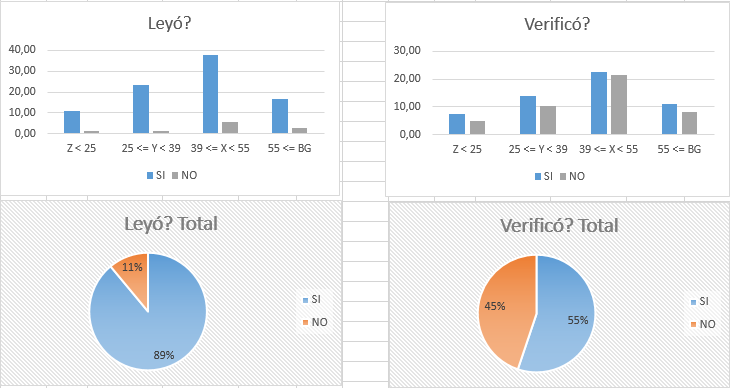
\includegraphics[width=\textwidth]{img/yfrjnCosp0.png}
  \caption{Comparación entre los que leen y verifican su boleta electrónica}
  \label{graf:votantes}
\end{figure}

Otro dato curioso de estas opiniones es que casi la totalidad de las personas les resulta sencillo su uso, sin embargo, muy pocas de ellas les genera confianza. Como se puede ver en el gráfico \ref{graf:votantesUsoConfia} la mitad de los encuestados les genera confianza o intentan confiar en este sistema. Sobre esta última característica destaca la variación de opiniones según la zona urbana encuestada, como se puede ver en la tabla \ref{tab:encuesta}, en el área centro (Escuela nº201)  se concentra la cantidad de personas que confían en sistema BUE, seguido del área Confluencia (Escuela nº40)  %\cambiar{Por otro lado las escuelas que se encuentran en zonas mas alejadas del centro no confían en este sistema. - HECHO}
Por otro lado las demás escuelas en zonas más alejadas del centro no logran confiar en este sistema. 
\begin{figure}[h!]
  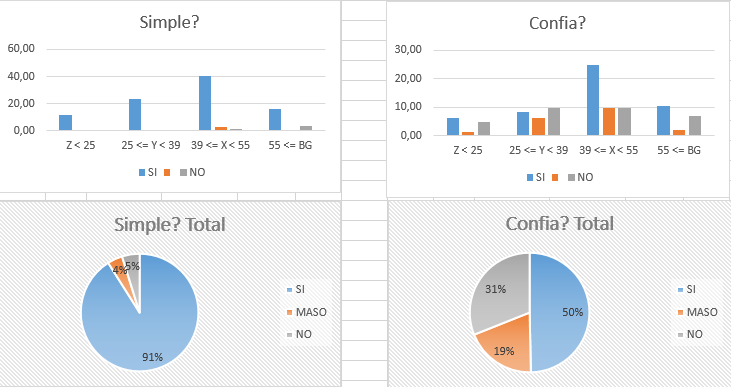
\includegraphics[width=\textwidth]{img/SLLXOorTia.png}
  \caption{Usabilidad vs. Confiabilidad}
  \label{graf:votantesUsoConfia}
\end{figure}

